\documentclass{article}
\usepackage{enumitem}
\usepackage{graphicx}
\usepackage{subcaption}
\usepackage{array}

\usepackage{color}
\usepackage[top=1in,bottom=1in,left=1.2in,right=1.2in]{geometry}
\usepackage{hyperref}
\usepackage[small]{titlesec}
\usepackage{booktabs}
\usepackage{colm2024_conference}
\usepackage{graphicx}
\usepackage[dvipsnames]{xcolor}
\usepackage{rotating}
\usepackage{pdflscape}
\usepackage{amsmath}

\newcommand{\todo}[1]{\textcolor{red}{\textbf{TODO:} #1}}

% Commenting
\newcommand{\eat}[1]{\ignorespaces}
%% Comment this line and uncomment the next to hide all comments
\newcommand{\xxcomment}[4]{\textcolor{#1}{[$^{\textsc{#2}}_{\textsc{#3}}$ #4]}}
\newcommand{\ta}[1]{\xxcomment{blue}{T}{A}{#1}}



\title{CS5787: Exercises 1 \\ \begin{small}\url{https://github.com/mitkrieg/dl-assignment-1/tree/main}\end{small}}
\author{Mitchell Krieger \\ mak483 \and \textbf{Meitong (Estelle) He} \\ mh2585}
\hypersetup{urlbordercolor=blue, linkcolor=blue, colorlinks=true}

\date{September 12, 2024}

\colmfinalcopy
\begin{document}
\maketitle

\section{Theory: Question 1 [12.5 pts]}

\begin{enumerate}[label=\alph*.]
    \item \textbf{What is the shape of the input $X$?} \\ There are $m$ samples in the batch with 10 features each so the input shape is $(m, 10)$ 
    \item \textbf{What is the shape of the hidden layer's weight vector $W_h$, and the shape of its bias vector $b_h$?} \\ To transform an $(m, 10)$ input into a hidden layer of 50 neurons we need a shape $W_h$ to have a shape of $(10, 50)$ so that we get a $(m, 50)$ result. After the weight matrix is applied, we then add the bias $b_h$ to each row of $W_hX$, which means that the $b_h$ needs to be $(1, 50)$
    \item \textbf{What is the shape of the output layer's weight vector $W_o$, and its bias vector $b_o$?} $W_h: (50, 3), b_h: (1, 3)$ using the same logic in part a, but now the hidden layer is the input and the output takes the place of the hidden layer.
    \item \textbf{What is the shape of the network's output matrix $Y$?} \\ The shape is $(m, 3)$ because there are m samples and three possible classes to have outputs for.
    \item \textbf{Write an equation that computes the network's output matrix $Y$ as a function of $X$, $W_h$, $b_h$, $W_o$, and $b_o$?}
    
          $Y = W_oa(W_hX+b_h)+b_o$ 

          Where $a$ is the ReLU activation funciton, $a(x) = \max(0,x)$.
\end{enumerate}

\section{Theory: Question 2 [12.5 pts]}

For the first layer there are 3x3x3 parameters in each of the 100 kernels, and then we need bias parameters for each kernel as well. This totals 3x3x3x100 + 100 = 2800 parameters. 

In the second layer there are 3x3x100 parameters in each of the 200 kernels, and then we need bias parameters for each kernel as well. This totals 3x3x100x200 + 200 = 180200. 

In the final layer there are 3x3x200 parameters in each of the 200 kernels, and then we need bias parameters for each kernel as well. This totals 3x3x200x400 + 400 = 720400. 

Adding all the layers together we get 2800 + 180200 + 720400 = 903400 total parameters.

\section{Theory: Question 3 [25 pts]}

\begin{enumerate}[label=\alph*.]
    \item
    \begin{equation*}
        \begin{aligned}
            \frac{\partial f}{\partial \gamma} &= \frac{\partial f}{\partial y_i} \frac{\partial y_i}{\partial \gamma} \\
            &= \sum_{i=i}^{m}\frac{\partial f}{\partial y_i} \widehat{x_i}
        \end{aligned}
    \end{equation*}
    \item        
    \begin{equation*}
        \begin{aligned}
            \frac{\partial f}{\partial \beta} &= \frac{\partial f}{\partial y_i} \frac{\partial y_i}{\partial \beta} \\
            &= \sum_{i=i}^{m}\frac{\partial f}{\partial y_i}
        \end{aligned}
    \end{equation*}  
    \item        
    \begin{equation*}
        \begin{aligned}
            \frac{\partial f}{\partial \widehat{x_i}} &= \frac{\partial f}{\partial y_i} \frac{\partial y_i}{\partial \widehat{x_i}} \\
            &= \frac{\partial f}{\partial y_i} \gamma
        \end{aligned}
    \end{equation*}  
    \item 
    \begin{equation*}
        \begin{aligned}
            \frac{\partial f}{\partial \sigma^2} &= \frac{\partial f}{\partial y_i} \frac{\partial y_i}{\partial \widehat{x_i}} \frac{\partial \widehat{x_i}}{\partial \sigma^2} \\
            &=  \sum_{i=i}^{m}\frac{\partial f}{\partial y_i} \gamma \frac{-1}{2} \frac{(x_i-\mu)}{\sqrt{(\sigma^2 + \epsilon)^3}}
        \end{aligned}
    \end{equation*}  
    \item 
    \begin{equation*}
        \begin{aligned}
            \frac{\partial f}{\partial \mu} &= \frac{\partial f}{\partial y_i} \frac{\partial y_i}{\partial \widehat{x_i}} \frac{\partial \widehat{x_i}}{\partial \mu} + \frac{\partial f}{\partial y_i} \frac{\partial y_i}{\partial \widehat{x_i}} \frac{\partial \widehat{x_i}}{\partial \sigma^2} \frac{\partial \sigma^2}{\partial \mu} \\
            &= \sum_{i=i}^{m}\frac{\partial f}{\partial y_i} \gamma \frac{-1}{\sqrt{(\sigma^2+\epsilon)}} \\
            &\quad+ \sum_{i=i}^{m}\frac{\partial f}{\partial y_i} \gamma \frac{-1}{2} \frac{(x_i-\mu)}{\sqrt{(\sigma^2 + \epsilon)^3}} \frac{-2}{m} \sum_{i=1}^{m}(x_i - \mu) 
        \end{aligned}
    \end{equation*}  
    \item
    \begin{equation*}
        \begin{aligned}
            \frac{\partial f}{\partial x_i} &= \frac{\partial f}{\partial \widehat{x_i}} \frac{\partial \widehat{x_i}}{\partial x_i} + \frac{\partial f}{\partial \sigma^2} \frac{\partial \sigma^2}{\partial x_i} + \frac{\partial f}{\partial \mu} \frac{\partial \mu}{\partial x_i} \\
            \frac{\partial f}{\partial x_i} &= \frac{\partial f}{\partial \widehat{x_i}}\frac{1}{\sqrt{\sigma^2+\epsilon}} + \frac{\partial f}{\partial \sigma^2}\frac{2}{m}(x_i-\mu) + \frac{1}{m}\frac{\partial f}{\partial \mu}\\
            \frac{\partial f}{\partial x_i} &= \frac{\partial f}{\partial y_i} \gamma \frac{1}{\sqrt{\sigma^2+\epsilon}} \\
            &\quad+ \frac{\partial f}{\partial y_i} \gamma \frac{-1}{2} \frac{(x_i-\mu)}{\sqrt{(\sigma^2 + \epsilon)^3}} \frac{2}{m}(x_i-\mu) \\
            &\quad+ \frac{1}{m}(\frac{\partial f}{\partial y_i} \gamma \frac{-1}{\sqrt{(\sigma^2+\epsilon)^3}} + \frac{\partial f}{\partial y_i} \gamma \frac{-1}{2} \frac{(x_i-\mu)}{\sqrt{(\sigma^2 + \epsilon)^3}} \frac{-2}{m} \sum_{i=1}^{m}(x_i - \mu) )
        \end{aligned}
    \end{equation*}
\end{enumerate}

\section{Practical [50 pts]}

In this experiment, our goal is to explore and compare the performance of three different regularization techniques for neural networks. We used the Lenet5 CNN architecture (\href{http://vision.stanford.edu/cs598_spring07/papers/Lecun98.pdf}{LeCun 1998}) as a baseline model trained on the FashionMNIST dataset. LeNet5 is composed of two convolutional layers with pooling after each convolution and then followed by three fully connected layers. 

\begin{table}[ht]
    \centering
    \begin{tabular}{|c|c|c|c|c|}
        \hline
        \textbf{Type} & \textbf{Kernels} & \textbf{Kernel Size} & \textbf{Padding} & \textbf{Output Shape} \\
        \hline
        Input         & -                & -                & -                     & 28x28x1 \\
        \hline
        Convolutional & 6                & 5x5              & 2                     & 28x28x6 \\
        \hline
        Max Pooling   & -                & 2x2 (Stride 2)   & -                     & 14x14x6 \\
        \hline
        Convolutional & 16               & 5x5              & 0                     & 10x10x16 \\
        \hline
        Max Pooling   & -                & 2x2 (Stride 2)   & -                     & 5x5x16 \\
        \hline
        Fully Connected & 120              & -              & -                     & 1x1x120 \\
        \hline
        Fully Connected & 84              & -               & -                     & 1x84 \\
        \hline
        Fully Connected & 10 (Classes)    & -               & -                     & 1x10 \\
        \hline
    \end{tabular}
    \caption{LeNet-5 Architecture with Layer Attributes}
    \label{tab:lenet5}
\end{table}


Note that we made a few small alterations to the original LeNet5 architecture. First, because the FashionMNIST image dimensions are different from the original dataset used by LeCun 1998 (28x28x1 instead of 32x32x1), we adjusted the input shape for this network. We also switched out the sigmoid activation function for ReLU and used max pooling instead of average pooling. This is because after running a few small manual tests we found that our models generally performed better on validation accuracy with these changes, and are less computationally expensive. In addtion, in the 25 years since LeNet5 was published, there has been research that has shown that these are these changes generally perform better (Krizhevsky, Sutskever, and Hinton 2012, Nair and Hinton 2010). Lastly we normalized the pixels in each image by diving element wise by 255. 

For this experiment, we tuned hyperparameters via a grid search training over possible combinations of hyperparameter values. Then we selected the model with the highest accuracy on a validation set that was created from an 80/20 random split of the training data. Model runs were logged in \href{https://api.wandb.ai/links/mitkrieger-cornell-university/dcihajq4}{weights and biases} for easy comparison. We first did this for the baseline architecture described above and then subsequently used the same method for each of the regularization techniques attempted. Table 2 describes each regularization experiment, the hyperparameters of the best model from the grid search, and the train and test accuracy after 25 epochs. Models were trained using cross entropy loss because this is a classification problem. Batch stochastic gradient decent (SGD) was chosen as an optimizer to speedup training over regular gradient decent. We used a batch size of 128 samples after manually experimenting a small handful of different sizes. This size was chosen because it was small enough to compute efficently, but still large enough to give a good sample size for the gradient to be estimated effectively from. We also attemped batch SGD with and without momentum to see if models would converge faster. For all models 25 epochs were used to be able to compare how they performed as training continued (even if models had seemingly converged at an earlier epoch).

\begin{table}[ht]
    \centering
    \caption{Hyperparameters for Regularization Experiments}
    \label{tab:lenet5}
    \begin{tabular}{|p{2cm}|p{3cm}|p{2cm}|c|c|c|}
        \hline
        \textbf{Technique}      & \textbf{Description}  & \textbf{Learning Rate}    & \textbf{Momentum}  & \textbf{Test Accuracy} & \textbf{Train Accuracy}\\
        \hline
        \raggedright No regularization       & \raggedright Standard model described above                     & 0.1                       & 0  & 0.09405 & 0.8988\\
        \hline
        \raggedright Batch Normalization     & \raggedright Two Batch normalization layers placed between each convolution and its activation as described by Ioffe \& Szegedy 2015.                  & 0.01                      & 0.9  & 0.0585 & 0.8964 \\
        \hline
        \raggedright Dropout                 & \raggedright Two Dropout layers placed between the first fully connected layer and the second, as well as the second fully connected layer and the output layer. A dropout rate of 0.2 was selected via grid search.                 & 0.1                      & 0  &0.9314 & 0.8996\\
        \hline
        \raggedright Weight decay            & \raggedright Weight decay was added to the batch SGD optimizer. A value of 0.001 was selected via grid search.                  & 0.01                      & 0.9 & 0.9165 & 0.8877\\
        \hline
    \end{tabular}
\end{table}

\newpage
Using the models above we can compare the performance of each technique. Figure 1 below holds the convergence graphs of the baseline's and each regularization experiment's test and train accuracies. In general, our test accuracies for all models reached a similar level at around 0.89.


\begin{figure}[ht] % Creates a floating figure
    \centering

    \caption{Convergence Graphs of Models}
    \label{fig:Convergence}

    % first row
    \begin{subfigure}[b]{0.45\textwidth}
        \centering
        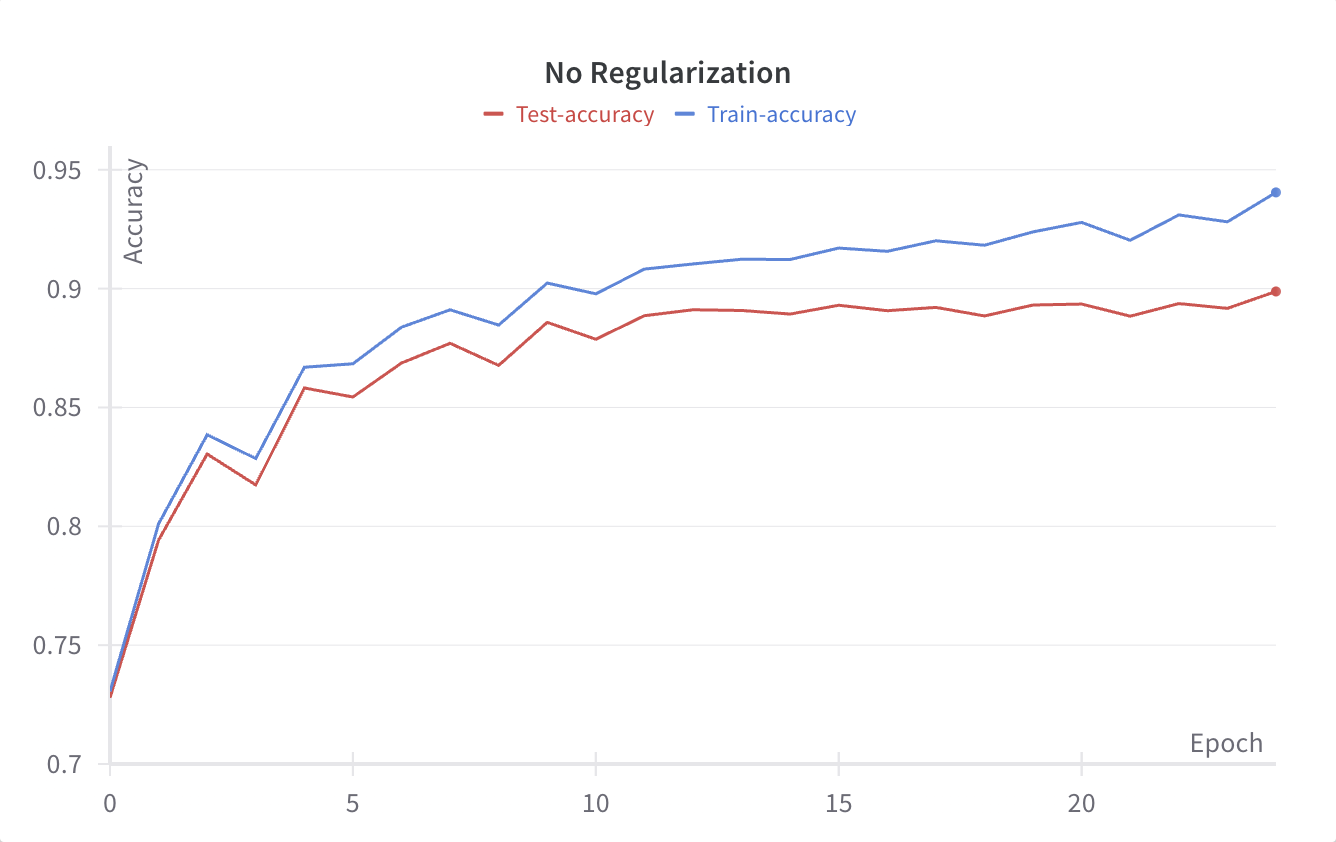
\includegraphics[width=\linewidth]{../src/no_reg.png}
    \end{subfigure}
    \hfill
    \begin{subfigure}[b]{0.45\textwidth}
        \centering
        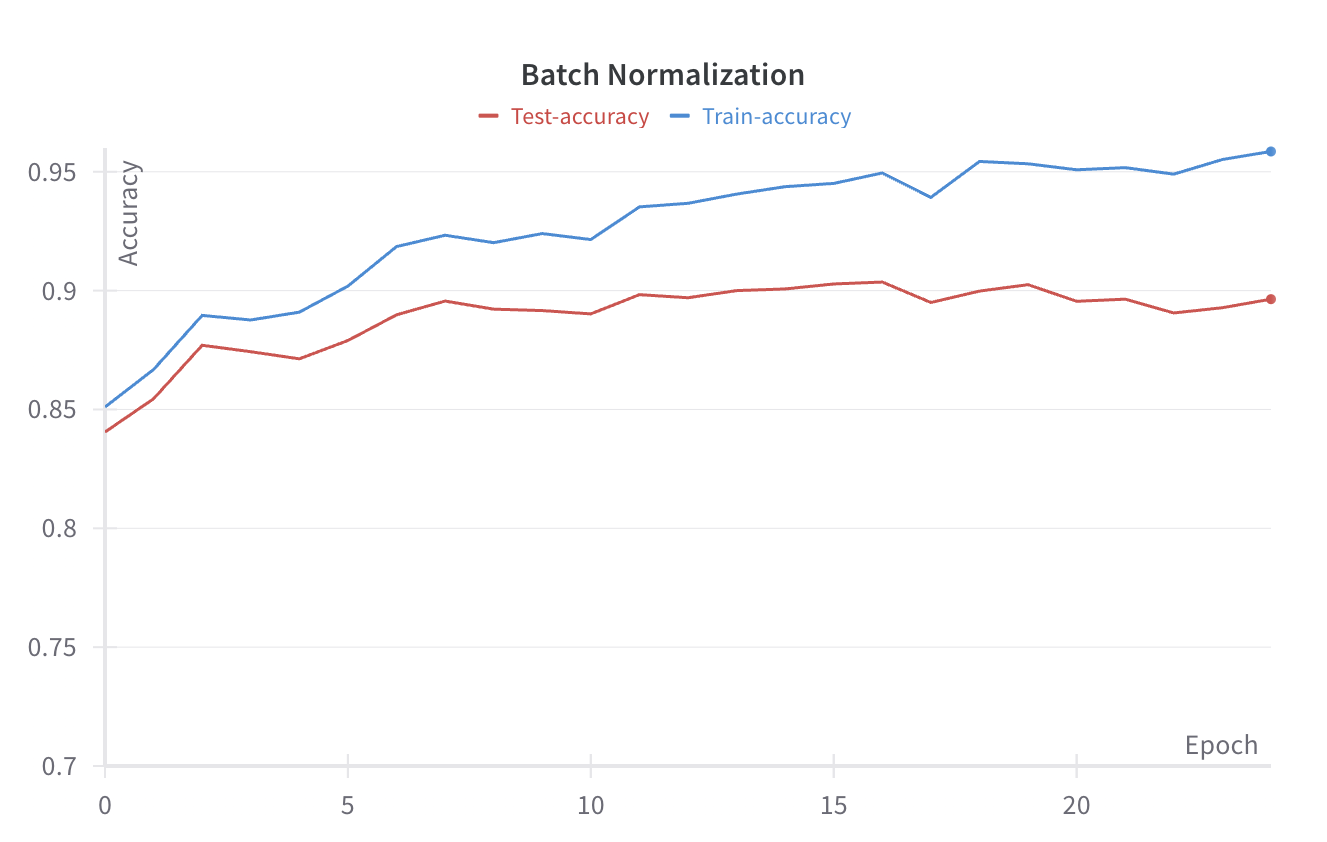
\includegraphics[width=\linewidth]{../src/batch_norm.png}
    \end{subfigure}
    
    % second row
    \vskip\baselineskip
    \begin{subfigure}[b]{0.45\textwidth}
        \centering
        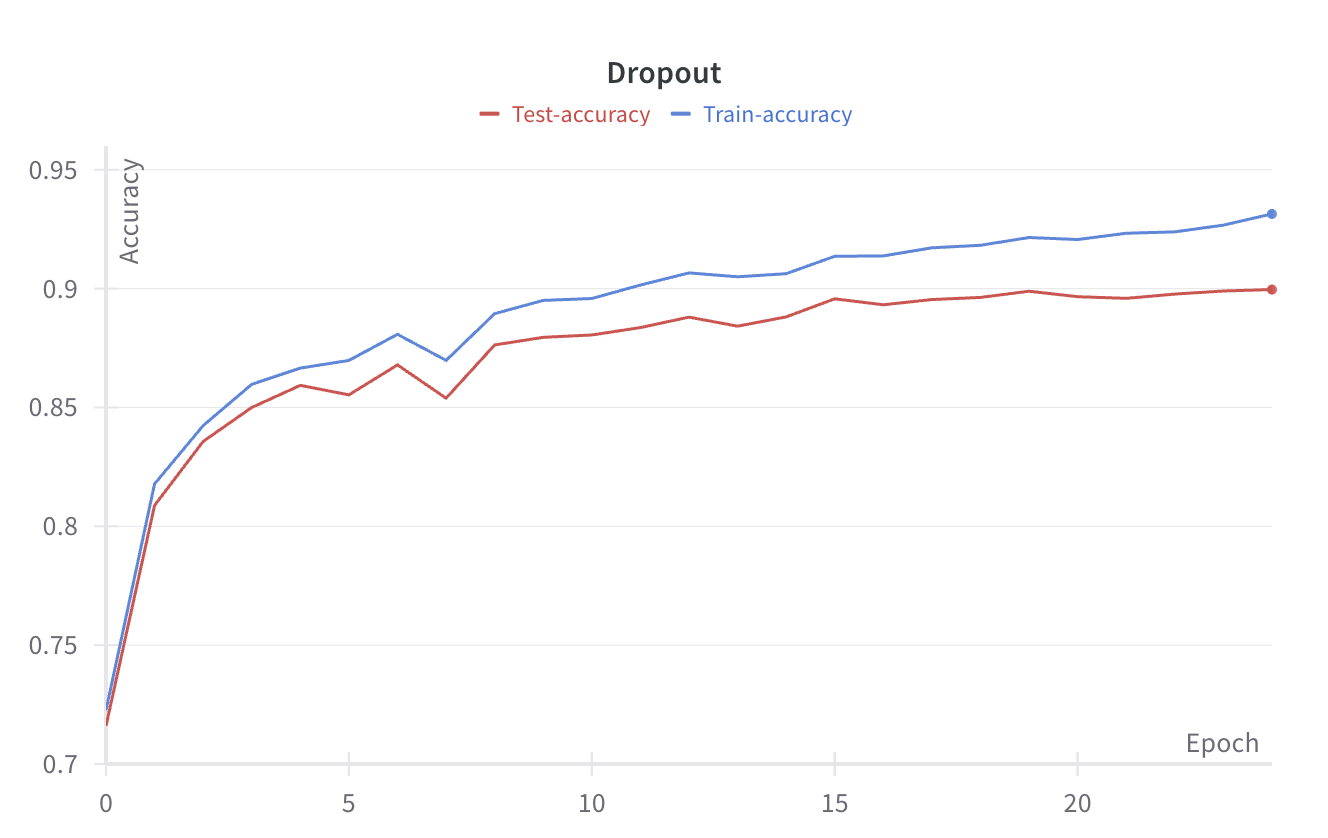
\includegraphics[width=\linewidth]{../src/dropout.png}
    \end{subfigure}
    \hfill
    \begin{subfigure}[b]{0.45\textwidth}
        \centering
        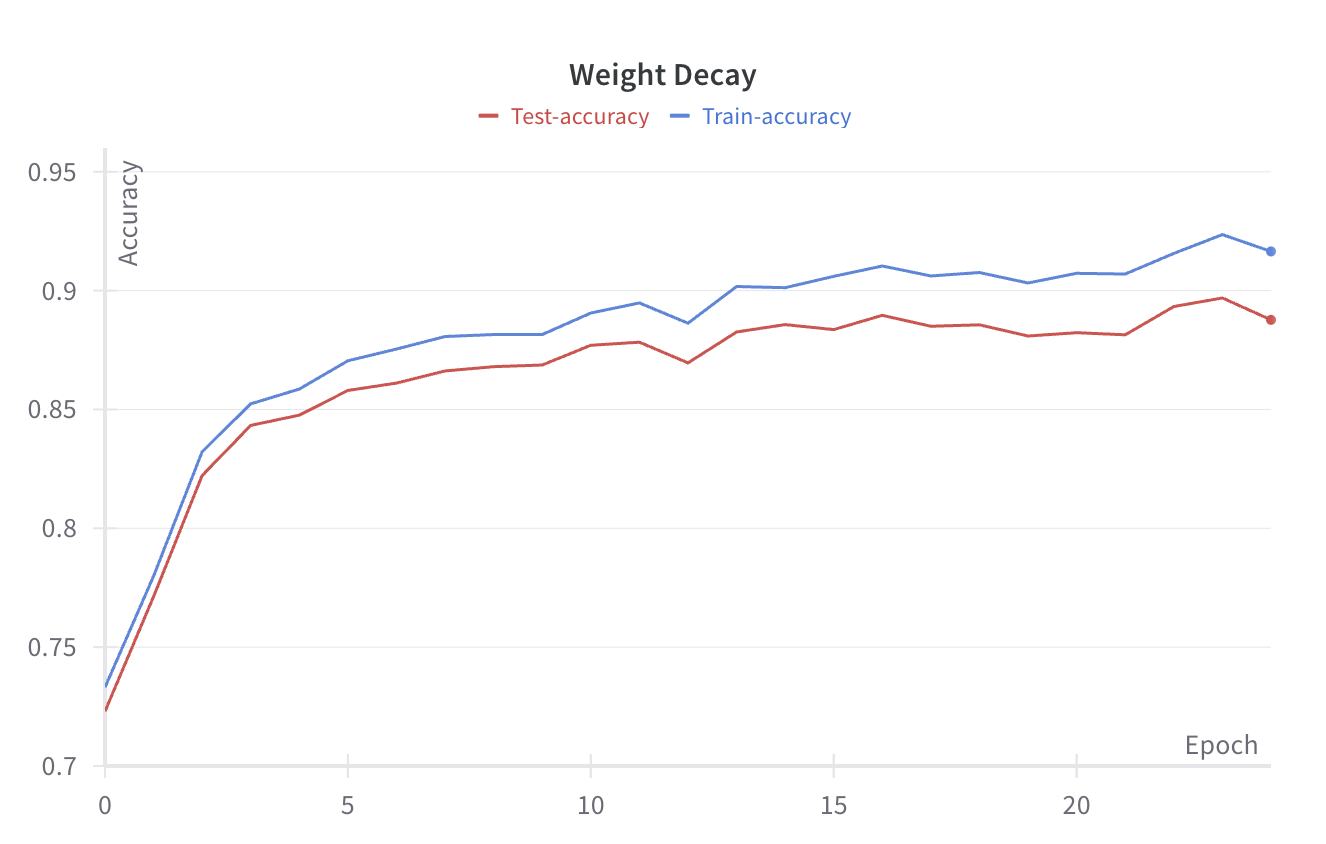
\includegraphics[width=\linewidth]{../src/weight_decay.png}
    \end{subfigure}
\end{figure}

The most visually apparent difference between the techniques is that batch normalization at the first epoch has an accuracy of around 0.1 higher than all other models and has the highest training accuracy. However, batch normalization also has the worst generalization error of any model inicated by the largest gap between the train and test lines in the final epoch. This potentially indicates that a) we allowed batch normalization to run for too many epochs and it over fit and/or b) that batch normalization as a technique learns quickly but is sensitive to the normed valued of the specific samples that were randomly chosen in each batch possibly leading again to over fitting. Both dropout and weight decay lessened the generalization error of the non-regularized model, illustrating that these methods are can be more effective in helping generalization, whereas batch normalization helps the model learn faster but is not as strong at curbing generalization error. 

In addition, both weight decay and dropout have smoother curves than the non regularized model and lower training accuracies. This demonstrates these techniques' ability weaken the power of batch SGD to take too big of a step in the direction of the gradient of one particular batch. During training with droupout we randomly remove some neurons and when we evaluate the train set. However during testing dropout is turned off for both the training and test set. This means we use all of the weights at inference but the weights of the neurons that were dropped out are dampened and ultimately, leading to better generalization while still learning features because of the removal of potential noise from the network. Weight decay or L2 regularization has a similar effect by adding the L2 penalty to the loss function. 

We can also see that all models had mostly converged around epoch 15, with batch normalizaiton converging fastest, deomnstraing that batch normalization helps with convergence because it stabilizes activations by reducing internal covariance shifts. Dropout on the otherhad, seems to convege the slowest, which makes sense because we are removing possible neurons to learn from. 

\end{document}
